\speciestitle{Hypochlorous Acid}{HOCl}{HOCl}{%
  \item[Useful range:] 10--2.2\,hPa
  \item[Contact:] Lucien Froidevaux, \email{Lucien.Froidevaux@jpl.nasa.gov}}

\subsection{Introduction}

There has been very little change in the \thisv HOCl retrieval results since \prevv, and any small changes are well within the somewhat large estimated accuracies (systematic uncertainties). We provide below sample mean HOCl distributions for the \thisv and \prevv data versions, and their differences. Otherwise, previous information regarding this species remains largely unchanged; the main points are mentioned here mainly for new data users.

The HOCl retrieval is quite noisy for individual profiles and HOCl data require some averaging (e.g., in 10\degsym\ zonal means for one or more weeks) to get useful precision of better than 10\,pptv, in comparison to typical upper stratospheric HOCl abundances of 100--150\,pptv. Table~\ref{tab:HOClSummary} summarizes the MLS HOCl resolution, precision, and accuracy estimates for the upper stratosphere. More discussion and a brief validation summary are given in the following sections, along with data screening recommendations. For trend results regarding MLS HOCl in the upper stratosphere, see \citep{FroidevauxEtal:2021:HOCl}.

An algorithm to retrieve daily zonal means of HOCl by first averaging the radiances has been developed by the MLS team, building on the work described in \citet{MillanEtal:2012} and \citet{MillanEtal:2015} for BrO and HO\cs2, respectively. This dataset reduces the variability slightly and will be available for \thisv from the GSFC DISC soon; it is expected to be very similar to the (\prevv) HOCl dataset used by \citep{FroidevauxEtal:2021:HOCl}. 

\subsection{Changes from \prevv}
There were no significant algorithmic changes relating directly to HOCl for the \thisv retrievals. However, given the small level of HOCl spectral radiance signal, the retrieved HOCl abundances can be sensitive, indirectly, to even minor changes in the retrieval system, such as changes in temperature or tangent pressure. In \prevv, small changes that likely contributed to HOCl differences included some changes to nitric acid in the R4 (640\,GHz) retrievals, in conjunction with (or tied to) changes from other bands (e.g., via differences in tangent pressure, temperature, and water vapor), and slight changes to a priori values for certain species (nitric acid, ozone, and water vapor).

The background observed in the 640-GHz radiances includes emissions from N\cs2, O\cs2, and H\cs2O. There are laboratory-based and ground-based models for the continuum absorptions that are the basis for the MLS absorption model \citep[][and references therein]{PardoEtal:2001}. These models were tested against MLS extinction measurements from the wing channels in the 640-GHz radiometer. The latitude dependence of this extinction was found to agree better with the expected moist plus dry continuum extinction values if the dry and moist continuum functions were scaled by factors close to 20$\%$; however, this aspect is no different than what was done in the previous data version.

A comparison plot showing zonal average upper stratospheric HOCl contours (from 10 to 2\, hPa) and differences between the two data versions for a typical month (April, 2009) is provided in Figure~\ref{fig:MLSv5v6HOClContour}. The average \thisv HOCl abundances are slightly larger than the \prevv retrievals, typically by about 10 to 15\, pptv (or 10 to 15$\%$); this has removed some of the small negative values that often occurred in \prevv HOCl contour plots at the highest southern latitudes, between 5 and 10\,hPa.  The estimated precision values are essentially unchanged from \prevv.

\begin{figure}
  \centering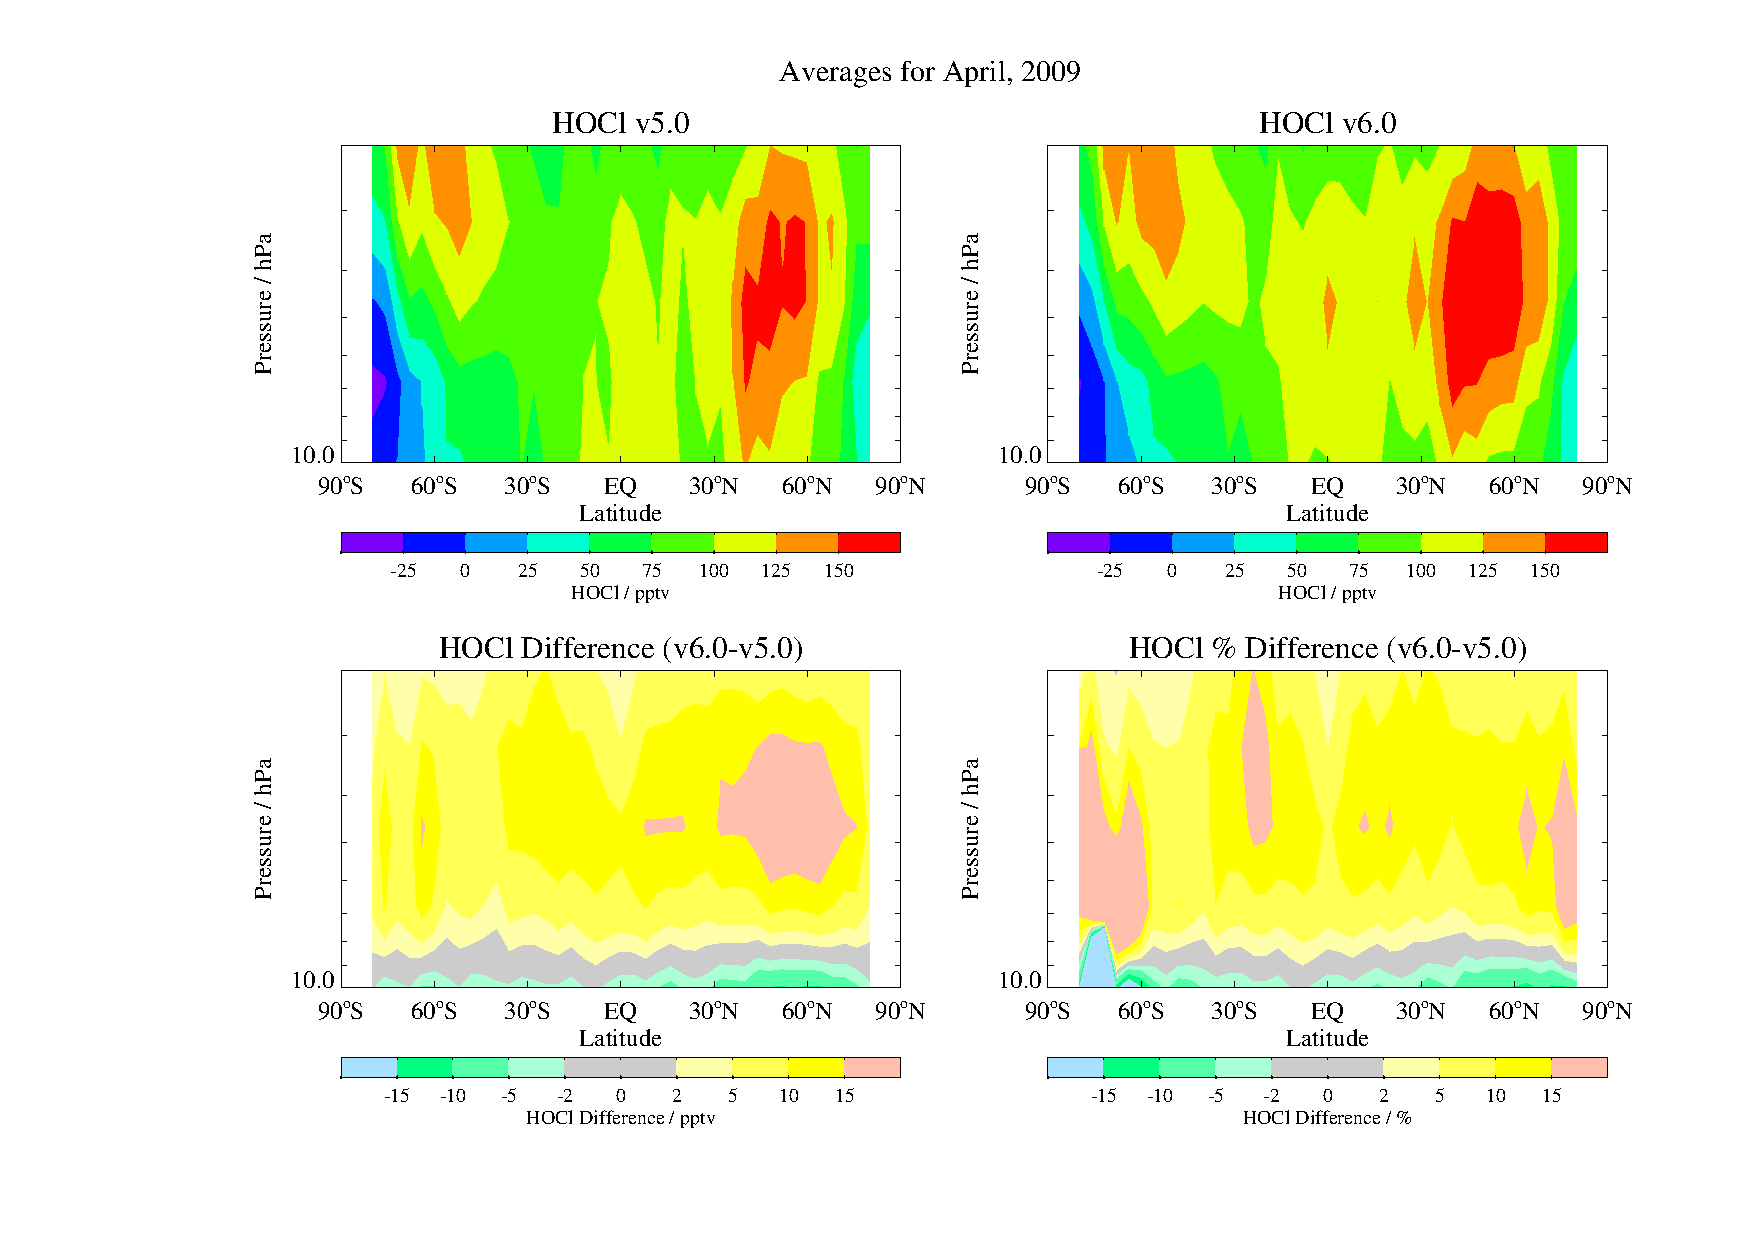
\includegraphics[angle=0,width=1.\linewidth]{figures/Fig-HOCl_v6v5_ZmContours_Difs.pdf}
  \caption{Zonal averages for upper stratospheric MLS HOCl profiles during April, 2009, showing the MLS \prevv HOCl mixing ratio contours (top left panel), the \thisv contours (top right panel), and their differences in pptv (\thisv minus \prevv, bottom left panel) and percent (\thisv minus \prevv versus \prevv, bottom right panel). }
  \label{fig:MLSv5v6HOClContour}
\end{figure}

\subsection{Resolution}
\oneverticalavk{HOCl}{HOCl}%

Based on the width of the averaging kernels shown in Figure~\ref{fig:AvkHOCl}, the vertical resolution for upper stratospheric HOCl is \mytexttilde6\,km (significantly worse than the 640-GHz radiometer vertical field of view width of 1.4\,km). This reflects the choice of smoothing constraints for HOCl which favor precision over vertical resolution.

\subsection{Precision}

The estimated single-profile precision reported by the Level~2 software is about 300 to 400\,pptv in the upper stratosphere. A more useful number of 5 to 10\,pptv is quoted in Table~\ref{tab:HOClSummary} for the typical precision of a 10\degsym\ weekly zonal means for this product.

\subsection{Accuracy}

The accuracy estimates shown in Table~\ref{tab:HOClSummary} come from a formal quantification of the combined effects of possible systematic errors in MLS calibration, spectroscopy, etc.\ on the HOCl retrievals \citep{ReadEtal:2007}. These values are intended to represent $2\sigma$ estimates of accuracy. The largest contributors to possible errors for HOCl are contaminant species, gain compression, and sideband ratio uncertainties. The Table gives a range of error estimates (for now, these are based on \prevv but they are not expected to change significantly). 
%The average changes for upper stratospheric HOCl between \prevv and \thisv are well within the quoted accuracy estimates (which may be somewhat conservative). The HOCl signal becomes too small compared to the systematic uncertainties to allow for reliable retrievals at pressures larger than 10 hPa.

\subsection{Data screening}
\label{sec:HOClScreening}
\begin{description}
  \item[Pressure range:] \screeningrule{10--2.2\,hPa} \standardrangestatement\ Artifacts (negative averages) for pressures larger than about 10\,hPa make this product unsuitable for use in the lower stratosphere. Regarding the topmost altitude range, the sensitivity to \emph{a priori} increases rapidly at pressures of 1\,hPa or less; we continue to recommend the use of (average) HOCl values only up to 2.2\, hPa. \standardprecisionrule \evenstatusrule

  \item[Quality field:] \screeningrule{Only profiles with a value of the \texttt{Quality} field \emph{greater} than 1.2 should be used.}
  This criterion removes profiles with the poorest radiance fits, typically less than 0.2$\%$ of the daily profiles. For HOCl, this screening correlates well with the poorly converged sets of profiles (see below); we recommend the use of both the \texttt{Quality} and \texttt{Convergence} fields for data screening.

  \item[Convergence field:] \screeningrule{Only profiles with a value of the \texttt{Convergence} field \emph{less} than 1.05 should be used.} For the vast majority of profiles (99$\%$ or more for most days), this field is less than 1.05. Nevertheless, on occasion, sets of profiles (typically one or more groups of ten profiles, retrieved as a `chunk') have this \texttt{Convergence} field set to larger values, and should be discarded.

  \item[Clouds:] \cloudsokrule

\end{description}

\subsection{Review of comparisons with other datasets}

The MLS HOCl retrievals exhibit the expected morphology in monthly mean latitude / pressure contour plots; for example, such plots for September months from MLS compare favorably, to first-order, with results produced by the Michelson Interferometer for Passive Atmospheric Sounding (MIPAS) for September, 2002 \citep{VonClarmannEtal:2006}. MLS HOCl averages at midlatitudes are close to the results from balloon-borne infrared measurements. Generally favorable comparisons (within the error bars) have been made of the diurnal changes in upper stratospheric HOCl between Aura MLS (v3.3), other satellite datasets, and a 1-D photochemical model \citep{KhosraviEtal:2013}.

\subsection{Artifacts}
\begin{itemize}
  \item The 640-GHz radiometer bands 10 (for ClO) and 29 (for HOCl) were turned off for a few time periods in 2006 to investigate degradation issues that might affect these channels in the future. These bands were off on April 8,9, and 10, 2006, and also for April 17, 2006 (after 19:52 UT) through May 17, 2006. There are essentially no useful HOCl (or ClO) data for these time periods. The \thisv (as for previous data versions) software correctly flags these incidents with poor (odd) \texttt{Status} values (which should be screened out).
  \item There are significant artifacts in the mean values (large negative values) for HOCl in the lower stratosphere, where the use of this product is not recommended.
  \item Users should screen out the non-converged and poorest quality HOCl profiles, as such profiles (typically a very small number per day) tend to behave unlike the majority of the other MLS retrievals. See the criteria listed above.
\end{itemize}

\begin{table}
  \caption{Summary for MLS hypochlorous acid}\vspace{0.5ex}
  \label{tab:HOClSummary}
  \begin{minipage}{\linewidth}\small
    \centering\begin{tabular}{ccccccl}
\toprule
\parbox[m]{15mm}{\centering\textbf{Pressure}} &
\multicolumn{2}{c}{\parbox[m]{16mm}{\centering\textbf{Precision\footnote{Precision ($1\sigma$) 
for 1 week/10 degrees zonal means or 2 weeks/5 degrees zonal means}}}} &
\parbox[m]{24mm}{\centering\textbf{Vertical\\ Resolution\\km}} &
\multicolumn{2}{c}{\parbox[m]{16mm}{\centering\textbf{Accuracy\footnote{$2\sigma$ estimate from systematic 
uncertainty characterization tests}\\}}} 
&
\textbf{Comments} \\
\textbf{hPa} & \textbf{pptv} & \textbf{\%} & \textbf{km}& \textbf{pptv} & \textbf{\%} & \\
\midrule
1.5 or less & ---   & ---   & ---    & ---    & ---     & Unsuitable for scientific use \\ 
2.2 to 10   & 5--10 & 5--20 & 5.5--6 & 40--80 & 25--100 & Some averaging required \\ 
15 or more  & ---   & ---   & ---    & ---    & ---     & Unsuitable for scientific use \\    
\bottomrule
\end{tabular}
  \end{minipage}
\end{table}
